\section{Introduction}

In software engineering, the task to translate from a language to another is very common. Modern programs depend on lots of library APIs, when those APIs change, usually many locations of the client programs need to be changed. Usually, APIs libraries are implemented and maintained in multiple languages. Taking an example with Lucene, a popular search engine, Lucene provides APIs that allows a third party client to access to its core features, thus there are a lot of Lucene clients that implemented in multiple languages such as Java, C\#, Python, etc. Lucene is originally implemented in Java, as a result, the Java client of Lucene is the version that needs to be evolved and maintained first, then the others come later. Thus the developer usually needs to keep an eye on the Java client while implementing another client, such as C\#, in order to synchronize the code of the clients. Because of such reason, there is a need for an approach to find translations between different languages, not only for the code structure but also for the semantics of the code.

Up to now, most of the focus has been spent on monolingual problems despite the existence of a wide variety of multilingual tasks. Recently, in the field of Natural Language Processing (NLP), the Neural Machine Translation (NMT) models have emerged as an alternative to statistical, phrase-based translation models, and achieved impressive translation performance. It raises a question: "\textbf{\textit{Can we build a Neural Machine Translation model for programming languages?}}"

\textbf{\textit{Our approach}}: Distributed vector representation has been successfully used to model natural languages and applied to problems such as neural machine translation, speech recognition, optical character recognition and others. One prominent distributed vector representation approach achieves significant attention is Word2Vec (Mikolov et al., 2013) \cite{mikolov2013distributed}, aka word embeddings. Word2vec, which is a neural-based language model, it is used for learning low dimensional vector representation of words, aka \textbf{embedding}. It uses language data to capture latent semantic features with respect to language modeling objective. The objective can be either to predict the context given a word or predict a word given a context

Our main goal is to produce good vector representation for tokens in language \textbf{across programming languages} by reducing this problem into a neural-based \textit{natural language processing} problem. Even though it has been observed that software has naturalness \cite{hindle2012naturalness} and statistical language models have been adapted to many software engineering tasks, such as code suggestions, code search, learning natural code convention, etc, it is not plausible to bring exactly the Word2Vec model for a cross-lingual programming language.  The main idea is to add a normalization step to in order to make the programming language to become natural-like, then we can find useful mappings between languages by learning a shared token embedding from the normalization data.

\textbf{\textit{Our contribution}}: The main contributions of this paper are:
\begin{description}
	\item [$\bullet$] We propose a novel way to add more natural-like semantics feature into programming languages, thus making it feasible to apply the neural-based natural language techniques to the programming language translation problem.
	\item [$\bullet$] We conduct large-scale evaluations on a different granularity of programming language to demonstrate the potential ability to use the neural-based technique for program translation through the program's elements mapping task.
	\item [$\bullet$] We prove that our work can be a benefit to real world task by evaluating our technique on a clone detection task. The data set is taken from on the diff data set from CLCMiner \cite{cheng2017clcminer} and we achieve a high precision and recall score. For the 10 projects in this dataset, the average precision is 85\% and the recall is 87\%.
\end{description}
\section{Background}

\subsection{Related work}
The Neural Machine Translation (NMT) models have emerged as an alternative to statistical, phrase-based translation models, and achieved impressive translation performance. The objective of NMT is to generate an appropriate sentence in a target language T given a sentence in the source language S. The NMT system first aggregates the vector representation of each word in the sentence through an encoder to build a "thought" vector, which is a sequence of number to represent the sentence meaning. and a decoder, then, processes the sentence vector to produce a translation. Here we can see that the foundation of such NMT models is the distributed vector representation of words, aka word embeddings.

The work of Hindle et al. \cite{hindle2012naturalness} yields a vision which suggests that techniques from natural language processing are useful in various programming tasks such as name suggestion, code completion, code search, etc. Miltiadis et al. \cite{allamanis2015suggesting} apply a neural-based model to the method naming problem. Raychev et al.\cite{raychev2015predicting} present a discriminative probabilistic model to predict types and names of variables in Javascript. Unfortunately, none of them have considered the language model for cross languages in software engineering.

\subsection{Background on Word2Vec}

Word2vec is a group of related models that are used to produce word embeddings. These models are shallow, two-layer neural networks that are trained to reconstruct linguistic contexts of words. Word2vec takes as its input a large corpus of text and produces a vector space, typically of several hundred dimensions, with each unique word in the corpus being assigned a corresponding vector in the space. Word vectors are positioned in the vector space such that words that share common contexts in the corpus are located in close proximity to one another in the space. Mikolov et al.\cite{mikolov2013distributed} introduce two variances of Word2Vec, which are Continuous Bag-of-Words (CBOW) and skip-gram. We show the skip-gram model in Figure 1 as we use it in our work.

\subsubsection{The skip-gram model}
The training objective of the skip-gram model is to find word representations that are useful for predicting the surrounding words in a sentence or a document. In other words, The skip-gram model aims to predict the word given the contexts. More formally, given a sequence of training words \begin{math}w_{1}, w_{2}, w_{3}, . . . , w_{T}\end{math}, the objective of the skip-gram model is to maximize the average log-probability:


\begin{displaymath}
J(\theta) = \frac{1}{T} \sum_{t=1}^T \sum_{-c\leq j\leq c,j\neq0} log(p(w_{t+j}|w_{t})
\end{displaymath}
where c is the size of the context window (which can be a function of the center word \begin{math}w_{t}\end{math}).

As described in (Mikolov at at.; 2013)\cite{mikolov2013distributed}, the skip-gram model (works well with small amount of the training data, represents well even rare words or phrases, while the Continuos Bag of Words model (CBOW) is several times faster to train than the skip-gram and slightly better accuracy for the frequent words. Since CBOW considers one target word and many context words, the task here is to predict the word given its context, it needs a bigger dataset to train for target vectors compared to datasets used in skip-gram. In other words, a dataset with short sentences but with a high number of samples is suitable for the CBOW model. On the other hand, the skip-gram model is designed to predict the context, so it needs a dataset with long sentences and a low number of samples due to many target words for single context word. In our case, a file (.java or .cs) are usually quite long, compare to a normal sentence in the Natural language, then the skip-gram is a more suitable model in this case. 


\subsubsection{ Parameters of the skip-gram model}
Here we want to give a brief explanation about the parameters that are being used for training with our data set.

\textbf{Negative sampling}: Training a neural network means taking a training example and adjusting all of the neuron weights slightly so that it predicts that training sample more accurately. In other words, each training sample will tweak all of the weights in the neural network. The size of the vocabulary means that our skip-gram neural network has a tremendous number of weights, all of which would be updated slightly by every one of our large number of training samples. Instead of taking the probability of the context word compared to all of the possible context words in the vocabulary, this method randomly samples 2-20 possible context words and evaluates the probability only from these. In other words, negative sampling addresses this by having each training sample only modify a small percentage of the weights, rather than all of them.

\textbf{Subsampling rate}: In a nutshell, subsampling is a method of diluting very frequent words, akin to removing stop-words. The subsampling method presented in (Mikolov et al., 2013) \cite{mikolov2013distributed} randomly removes words that are more frequent than some threshold \textit{t} with a probability of \textit{p}.

\textbf{Window size}: The window size is randomly chosen between 1 and max size for each training sample, resulting in words with the maximum distance being observed with a probability of 1/c while words directly next to the given word are always observed. For example, if the window is set to 5 then for the current word w surrounding 10 words will be taken as context words.



\begin{figure}[t!]
	
	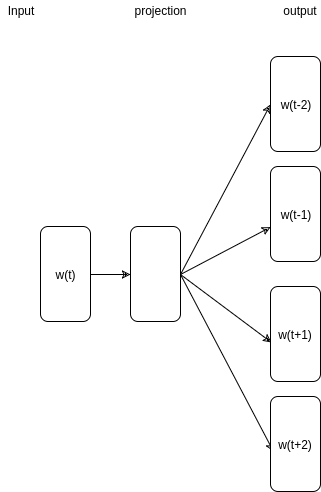
\includegraphics[width=0.20\textwidth]{skipgram}
	\caption{The Skip-gram model architecture. The training objective is to learn word vector representations that are good at predicting the nearby words.}
	\label{fig:clf}
\end{figure}

\subsection{Billingual embedding models}
The bilingual embedding models capture not only semantic information of monolingual works but also semantic relationships across different languages. Here we want to describe briefly the bilingual modes in the field of Natural Language Processing, thus the differences between them affect the choice in our framework. We can categorize approaches to learn bilingual word representation in 3 different schemes: bilingual mapping, monolingual adaptation, and bilingual training.
\begin{description}
	\item [$\bullet$] \textbf{Billingual Mapping}: First, word representations are obtained on each language independently, either by CBOW or skip-gram model. This method assumes that alignment information at word-level between languages are available, e.g: the(English) - le(French), dog(English) - chien(French). As described in \cite{mikolov2013exploiting}, the vector representations of similar words in different languages are related by a linear transformation, as they have similar geometric arrangements. Given the word representations for two language \begin{math}l_{1}\end{math} and \begin{math}l_{2}\end{math} that are learned independently and the alignment information are available, the goal of this method is to learn a transformation matrix \textit{W} such that \begin{math}W l_{1}\end{math} approximates \begin{math}l_{2}\end{math}.
	\item [$\bullet$] \textbf{Monolingual Adaptation}: this scheme, on the other hand, only need the vector representations for the source language and the alignment information at word-level. The goal is to bootstrap learning of target representations and make sure the target representations of semantically similar words across languages are close together. Zou et al. (2013) consider the unsupervised alignment information derived from a parallel corpus.
	\item [$\bullet$] \textbf{Billingual Training}: the previous schemes assume fixed pretrained representations on either one or both sides. This scheme attempts to jointly learn representations from scratch. The Bilingual skip-gram model (BiSkip), proposed by (Thang et al., 2015) \cite{luong2015bilingual}, utilizes only the alignment information between languages to learn good vector representations for both languages. This work has carefully examined the quality of the learning bilingual embeddings, while the others have not.
\end{description}
Our goal in this paper is to learn a good vector representations for cross programming languages, we also want to keep a good vector representation for each language separately. The BiSkip model is proved to perform outstanding both in bilingual tasks and monolingual tasks \cite{luong2015bilingual}, compares to the others.

\section{Our Approach}
\subsection{Overview}

\begin{figure*}[t!]
	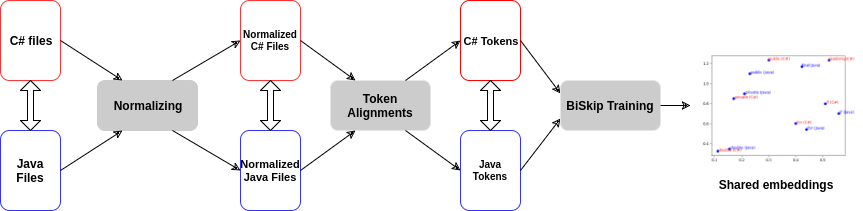
\includegraphics[width=0.60\textwidth]{approach}
	\caption{An overview of our framework}
	\label{fig:approach}
\end{figure*}



Figure \ref{fig:approach} is the overview of our approach. There are 4 steps:
\begin{description}
	\item [$\bullet$] \textbf{Files alignment}:In order to train the BiSkip model, we need the parallel corpus of languages. We collect data from open-source projects cross-lingually and get the aligned files. The process to get the aligned files are shown in section 4.1.
	\item [$\bullet$]\textbf{Data Normalizing}: This is the key step to get a better shared embedding by adding more semantic meanings to the training data. This step is comprised of 3 steps: preprocessing, adding semantic information and postprocessing the data.
	\item [$\bullet$] \textbf{Token Alignment}: Before learning the shared embeddings cross-lingually, we need to get the token alignment information. In our case, we do not have the monotonic token alignments. In addition, not like the natural language, the tokens in a programming language can be anything, except some language keywords, e.g: \texttt{if, for, while, public}, etc. So we utilized existing unsupervised token alignment techniques proposed by Liang \cite{liang2006alignment}.
	\item [$\bullet$] \textbf{BiSkip Training}: Once we get the token alignments information, we use it to learn shared embedding for all tokens in both languages. The vector representations after learned are used to describe the semantic meaning of tokens among the others.
	
	
\end{description}




\subsection{Data Normalization}
\label{sub:normalization}
In natural language processing, the data normalization step is a process to remove uninteresting contents from the data set and transform the rest into normalized comparison units. In our case, we are performing on the similar task for programming languages. The differences between the programming language and natural language can be described as:
\begin{description}
	\item [$\bullet$] Programming languages are formally defined, there is a mathematical definition of their semantics.
	\item [$\bullet$] Vocabulary of programming languages is very limited and restricted to a few number of words in a very specific domain. The vocabulary, in this case, is language keywords, eg. if, else, for, while, etc.
	\item [$\bullet$] Programming languages are perfectly unambiguous and have bounded and precisely defined vagueness.
\end{description}
Because of such differences, usual techniques to process natural language may not provide enough usefulness for programming language processing task.
Besides removing uninteresting contents, we add more semantic features into training corpus with the intuition that these features are able to remove the syntactic gap between languages. This is the key step to learn the embedding cross-lingually. This process involves 3 sub-processes:

\begin{description}
	\item [$\bullet$] \textbf{Pre-processing}: We remove all of the useless information such as comments, special character, but not all of them. In order to keep as many semantic meanings as we can, we treat the operators as tokens that also need to learn the embeddings. Usually, the operators will be similar to the special character, to distinguish between them, we adopt srcML \cite{collard2011lightweight} to parse the source code, so we can identify if a token is a language operator or just a special character
	\item [$\bullet$] \textbf{Adding semantic information}: Once we get the XML representation of the source code, we have the information of each element from the codes, we traverse the XML representation to add or replace code elements with predefined keywords to add more semantic meaning to the raw source code. We selectively present some of the rules to add or replace code elements with keywords in Table 1.
	\item [$\bullet$] \textbf{Post-processing}: Once we get the enhanced semantic version of the code, the camel case tokens and tokens with underscores are split by upper case letters and the underscore to reduce differences between programming styles.
\end{description}

\begin{figure}[t!]
	
	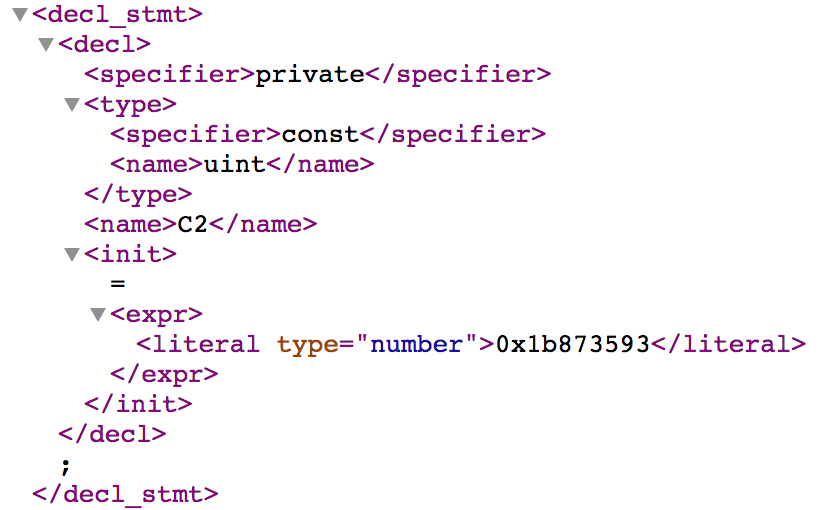
\includegraphics[width=0.3\textwidth]{srcml_sample}
	\caption{SrcML sample}
	\label{fig:srcml_sample}
\end{figure}

In Table 1, we selectively pick out some typical elements of programming languages to demonstrate our data normalizing process, the examples provided in the Table can be written either in \text{C\#} or Java. Taking an example, we have the code fragment: 

\begin{lstlisting}
for(int i = 0; i < 10; i++)
\end{lstlisting}

which is a simple for loop with three elements, the initialization part, the condition part and the afterthought part. We apply rule 5 into the initialization part, which transforms the variable \textbf{i} into the fixed keyword \textbf{identifier}. Then we apply rule 5 and rule 8 to the condition part, by transforming \textbf{i} into \textbf{identifier} and \textbf{10} to \textbf{literal\_type number}. Finally, we apply rule 13, rule 9 to add the keyword \textbf{operator} before \textbf{++}. 

\begin{table*}
	
	\label{tab:freq}
	\resizebox{\textwidth}{!}{
		\begin{tabular}{p{2cm}|p{0.79cm}|p{2cm}|p{3cm}|p{4cm}|p{4cm}}
			
			\hline
			\textbf{Element}&\textbf{Index} &\textbf{Sub-Element}&\textbf{Rule}&\textbf{Example code}&\textbf{Applied Rules}\\
			
			\hline
			Statements & 1&if statement & add \textbf{condition} & \texttt{if(x$>$5) y+=4} & if expr type int identifier operator $>$ literal\_type number expr\_stmt expr identifier operator += literal\_type number\\\cline{2-6}
			
			&2& for statement & add \textbf{condition}, \textbf{control} & \texttt{for(int i=0;i$<$10;i++)}  & for control init type int idenfier operator = number condition expr identifier operator $<$ literal\_type number identifier operator ++\\\cline{2-6}
			
			&......&&&& \\\cline{2-6}
			
			\hline
			Expressions &3& function call & add \textbf{call} & \texttt{Console.WriteLine("out")}  & expr\_stmt expr call Console Write Line argument literal\_type string\\\cline{2-6}
			
			&......&&&& \\\cline{2-6}
			
			\hline
			Declarations, Definitions and Initializations &4& variable declaration statement& add \textbf{decl\_stmt} & \texttt{int i} & decl\_stmt decl type int identifier\\\cline{2-6}
			
			&5& variable identifier definition & replace with \textbf{identifier} & \texttt{string s}& string identifier\\\cline{2-6}
			
			&6& function declaration & add \textbf{function\_decl} & \texttt{void doWork()}& function\_decl void do Work \\\cline{2-6}
			&......&&&& \\\cline{2-6}
			\hline
			Others &7& inheritance list & add \textbf{super} & \texttt{class Foo: Bar \{ \}} & class Foo super Bar\\\cline{2-6}
			
			&8& literal & add \textbf{literal\_type} & \texttt{int x = 9}& int identifier operator = literal\_type number \\\cline{2-6}
			
			&9& operator & add \textbf{operator} & \texttt{a \& b }&  identifier operator \& identifier \\\cline{2-6}
			&......&&&& \\\cline{2-6}
			
			
			\hline
	\end{tabular}}
	\medskip
	\caption{Source code Transformation Rules - For each type of elements, we define subtypes of it and we manually define rules to add more semantic keywords to the code. The code after adding the sematic keywords become a natural-like sentence.}
\end{table*}


\begin{figure}[t!]
	
	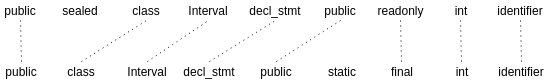
\includegraphics[width=0.48\textwidth]{alignment}
	\caption{Sample alignment of code fragments between \text{C\#} and Java code, both the fragments have already been normialized.}
	\label{fig:alignment}
\end{figure}

\subsection{The Bilingual skip-gram Model}

Our final goal is to build a shared embedding vector space cross-lingually. We use the bilingual skip gram model (BiSkip) \cite{luong2015bilingual} to achieve this goal. The BiSkip is an extension of the skip-gram model, the motivation behind the BiSkip is to learn a shared embedding space between tokens cross-lingually rather than just learning monolingually in the skip-gram model. Rather than just predicting the tokens in the source language, they use the tokens in the source language to additionally predict their aligned tokens in the target languages. Imagine that if we know that the token \textit{readonly} in \text{C\#} is aligned to and has the same meaning as the token \textit{final} in Java in Figure 5, we can simply substitute \textit{readonly} and use \textit{final} to predict the surrounding tokens such as \textit{int} and \textit{public}. 

Given an alignment link between a token $t_{1}$ in a language $l_{1}$ and a token $t_{2}$ in another language $l_{2}$, the BiSkip model uses the token $t_{1}$ to predict the surrounding tokens of the token $t_{2}$ and vice versa. We can think of this BiSkip model as training four skip-gram models jointly which predict tokens betwwen the follow pairs of languages: $l_{1} \rightarrow l_{1}, l_{2} \rightarrow l_{2}, l_{1} \rightarrow l_{2}, l_{2} \rightarrow l_{1}$.

\subsubsection{ Unsupervised token alignment}

Once we finish normalizing our training data, we want to learn a shared embedding space between tokens cross-lingually rather than just monolingually. In order to do that, we need to obtain aligned information from such languages. We do not have the alignment information, thus the alignment information must be obtained to the unsupervised manner. We briefly review the sequence-based unsupervised token alignment models. Generally, the token alignment model are generative models of the form p(\textbf{t $|$ s}) = $\displaystyle\sum_{a} p(\textbf{a,t $|$ s})$, where $\textbf{s} = (s_{1},..., s_{J})$ is the source sentence, $\textbf{t} = (t_{1},..., s_{J})$ is the target sentence and $\textbf{a} = (a_{1},..., a_{J})$ is the asymmetric alignment which specifies the position of a token in source language aligned to each target language. Berkeley aligner (Liang et al. \cite{liang2006alignment}) is a joint training approach, while the source language and target language play a symmetric role in the word alignment task, sequence-based models are asymmetric,they are generative models of the form p(\textbf{t $|$ s})(S $\rightarrow$ T) or p(\textbf{s $|$ t})(T $\rightarrow$ S) by reversing the roles of source and target. This suggests that two models make different types of errors that can be eliminated upon intersection. Figure 4 shows an example alignment of tokens of code fragments between \text{C\#} and Java code as an output of the Berkeley aligner.

\begin{figure}[t!]
	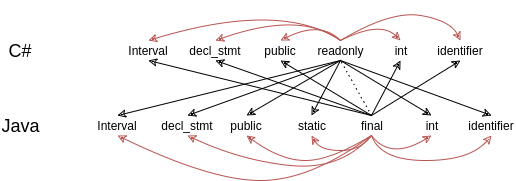
\includegraphics[width=0.35\textwidth]{biskip_align}
	\caption{Billingual Skipgram Model - besides predicting within languages, the model also predict crosslingually based on the alignment information. From the output of the unsupervised token alignment, the token \textit{readonly(C\#)} and \textit{final(Java)} are aligned, then use the \textit{readonly} to predict the surrounding contexts of itself and target language, and vice versa for the token \textit{final}.}
	\label{fig:clf}
\end{figure}

\section{Experiments}


\subsection{Data}
We collect data from 10 open source projects cross-lingually in C\# and Java. With the intuition that the different implementations of the same project in different languages contain the same logical information, thus files with the same indicator also contain the same logical information, so they are aligned to each other. In natural language processing, such information is called aligned sentences or aligned documents. Here we call them aligned files. Taking Lucene as an example, the file \texttt{AbstractEncoder.cs} under C\# Lucence Client project has the same indicator \texttt{AbstractEncoder} with the file \texttt{AbstractEncoder.java} under Java Lucene Client project, so they are aligned to each other. We get around 13770 pairs of aligned implementation over 10 projects and we normalize all the pairs. Table 2 is an overview of our training data set.

\begin{table*}
	
	
	\resizebox{\textwidth}{!}{
		\begin{tabular}{c|cc|cc|cc|cc|cc|cc|cc|cc|cc|cc}    
			\hline
			Projects&
			\multicolumn{2}{c}{aws-sdk} &
			\multicolumn{2}{c}{antlr} & \multicolumn{2}{c}{datasax} & \multicolumn{2}{c}{factual} & \multicolumn{2}{c}{fpml} & \multicolumn{2}{c}{log4j/4net} & \multicolumn{2}{c}{lucene} & \multicolumn{2}{c}{spring} & \multicolumn{2}{c}{zeromq} & \multicolumn{2}{c}{mongodb}  \\
			\hline
			Languages&C\# & Java&C\# & Java &C\# & Java &C\# & Java &C\# & Java &C\# & Java &C\# & Java &C\# & Java &C\# & Java &C\# & Java \\
			\hline
			Files& 18801 & 23503 & 593 & 351  & 545 & 548 & 55 & 63 & 124 & 124 &293 & 298 & 2709 & 5703 & 2364 & 5697 & 206 & 220 & 1914 & 1087 \\
			\hline
			Aligned files& \multicolumn{2}{c|}{9850}&\multicolumn{2}{c|}{205} & \multicolumn{2}{c|}{98}  & \multicolumn{2}{c|}{35} & \multicolumn{2}{c|}{140} & \multicolumn{2}{c|}{78} & \multicolumn{2}{c|}{2445} & \multicolumn{2}{c|}{550} & \multicolumn{2}{c|}{89} & \multicolumn{2}{c}{280} \\
	\end{tabular}}
	\caption{Overview of our training data set}
	\label{tab:dataset}
\end{table*}
\begin{figure}[t!]
	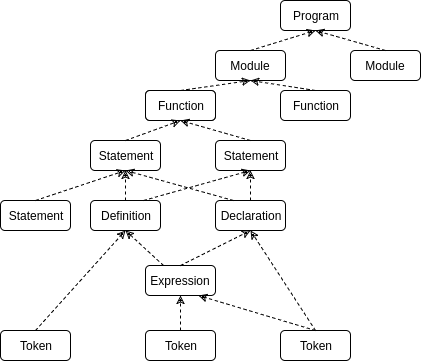
\includegraphics[width=0.44\textwidth]{software_layers}
	
	\caption{Software layers - shown are the hierarchical layer architecture of elements in software.}
	\label{figure:softwarelayers}
	\medskip
\end{figure}
\subsection{Training}
We use the following settings: stochastic gradient descent with a default learning rate 0.025, negative sampling with 30 samples, skip-gram with context window of size 10, and a subsampling rate of value 1e-4. All models are trained for 10 epochs and the learning rate is decayed to 0 once training is done. In Natural Language, according to \cite{pennington2014glove}, the number of words is usually large in the training set and we need a large dimension (range from 100 to 300) to capture the whole semantic meaning of the words. In our case, our training set is relatively smaller, so we choose 50 as the dimension size.
\subsection{Evaluation Tasks}
We evaluate our metho on 3 tasks: tokens mapping, elements mapping and clone detection. These 3 tasks represent for different granularities of programming language structure. Consider Figure \ref{figure:softwarelayers}, a program is usually constituted of different modules. A module could have a set of related functionalities and a functionality is represented as a set of classes. A class comprises of methods and a method comprises of smaller elements, such as expression, and statement. Thus a software program can be visualized as a hierarchical layer architecture of elements. Here we want to evaluate the effectiveness of our approach when mapping elements in cross languages in different granularities. In the tokens mapping task, we want to evaluate how effective our model is on the token level, the mapping at this level is important because this is served as a based level for a more high-level representation of source code. The elements mapping task represents a more coarse-grained level of source code. Formally, an element, such as expression, declaration or statement is a \textbf{semantic composition} of tokens in a structural way. Finally, we evaluate our approach by comparing the similarity of some "big" code fragments. We use the diff data set from \cite{cheng2017clcminer}, which contains the code hunk from the revision history, so called \textit{diff}. These may not complete code fragments but still, contain some structural and semantic meaning.
\subsubsection{Tokens mapping}
This task measures the semantic quality of the learned token vectors cross-lingually.  We manually defined the token-level alignment list between languages'as the ground truth. The types of tokens to be considered are the language keywords and the operator symbols (such as \&\&,$+$,$+=$, etc). For example, \textbf{\textit{readonly(C\#)}} should be aligned to \textbf{\textit{final(Java)}}. Then for each C\# keyword in the list, we take out the vector representation of that keyword in the C\# vector space, we use that keyword as the query to find k-nearest neighbors of that key word in the Java vector space based on Euclidean distance, we do this task in both directions, from C\# to Java, and from Java to C\#. 

Once we get the results, we calculate the Average Precision of that query. 
The Average Precision can be calculated as follow:
\begin{displaymath}
AP = \frac{\prod_\text{k=1}^n P(k)*rel(k)}{d}
\end{displaymath}
where P(k) is the precision at cut-off k in the list, rel(k) is an indicator function equaling 1 if the item at rank k is a relevant document, zero otherwise and d is the number of relevant documents.

Once we get the AP for each query, we then calculate the Mean Average Precision for all queries. The MAP can be calculated as follow:
\begin{displaymath}
AP = \frac{\prod_\text{p=1}^Q AP(q)}{Q}
\end{displaymath}
where q is the query, and Q is the number of total queries.
\begin{figure*}[t!]
	\centering
	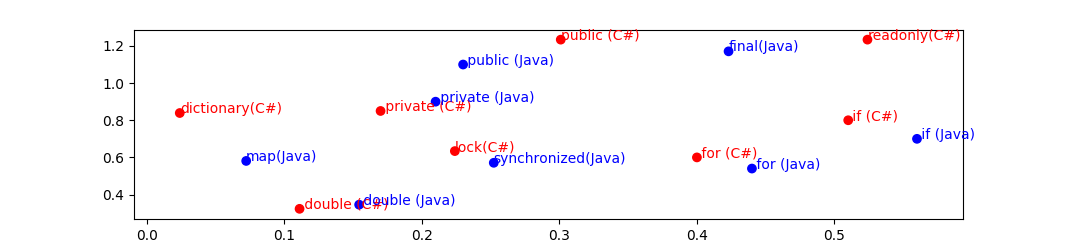
\includegraphics[width=1\textwidth]{example_bi2vec_tsne}
	\caption{A visualization of shared embeddings between \text{C\#} and Java under t-sne. The node with red text are the tokens from C\#, the blues are from Java. The tokens that serve the same function for both languages should be close to each other.}
	\label{fig:tsne}
\end{figure*}

\begin{figure*}[t!]
	\centering
	
	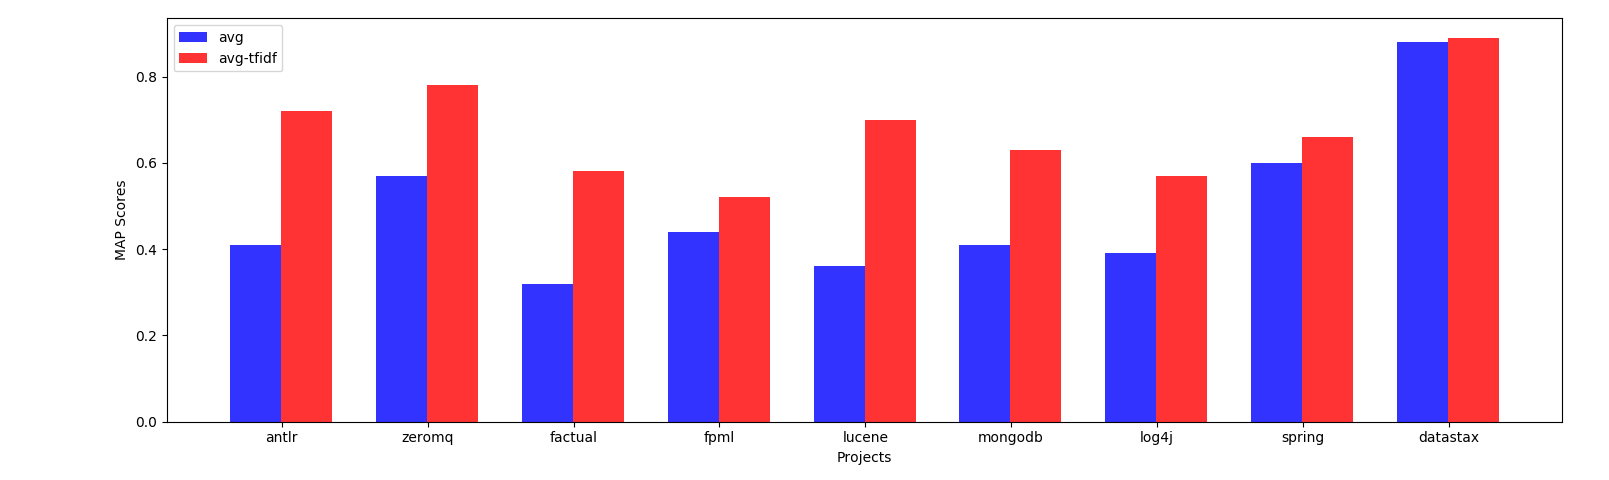
\includegraphics[width=1.05\textwidth]{avg_vs_tfidf}
	\caption{Performance comparision of \textit{avg} and \textit{avg-tfidf} for the method mapping task. The y axis is the MAP score taken from top-5 queries for each project. The \textit{avg-tfidf} significantly boosts the MAP score and outperform the \textit{avg}.}
	\label{fig:avg_vs_tfidf}
\end{figure*}



\begin{table*}
	
	
	\resizebox{\textwidth}{!}{
		
		\begin{tabular}{c|c|c|c|c|c|c|c|c|c|c|c|c}
			
			
			Element & \multicolumn{4}{c|}{Expression}  & \multicolumn{4}{c|}{Statement} & \multicolumn{4}{c}{Method} \\
			\hline
			Language& \multicolumn{2}{c|}{C\#} & \multicolumn{2}{c|}{Java} & \multicolumn{2}{c|}{C\#} & \multicolumn{2}{c|}{Java}& \multicolumn{2}{c|}{C\#} & \multicolumn{2}{c}{Java}\\
			
			\hline
			Approach& avg & avg-tfidf & avg & avg-tfidf & avg & avg-tfidf & avg & avg-tfidf & avg & avg-tfidf & avg & avg-tfidf\\
			
			\hline
			antlr  &0.43 &0.56 & 0.51 &0.67 &0.32 &0.47 & 0.37 & 0.53 & 0.38& 0.44 & 0.25 & 0.41\\
			lucene  &0.44 &0.51 & 0.33 &0.70 &0.28 &0.61 & 0.38 & 0.48 & 0.34 & 0.70 & 0.31 & 0.51\\
			factual  &0.38 &0.58 &0.40 &0.69 &0.27 &0.56 &0.44 & 0.32 &0.36 &0.48 &0.39 & 0.44 \\
			zeromq   &0.43 &0.69 & 0.44 &0.73 &0.45 &0.65 &0.50& 0.68 & 0.59 & 0.72 & 0.59 & 0.70\\
			datastax &0.66 &0.70 &0.51 &0.55 &0.56 &0.58 & 0.85 &0.86 &0.76 &0.82 &0.76 & 0.84 \\
			mongodb &0.34 &0.59 &0.45 & 0.49 &0.64 &0.52 &0.54 & 0.55 & 0.41 & 0.62 & 0.51 & 0.58  \\
			fpml   &0.47 & 0.49 &0.55 &0.35 &0.42 & 0.55 &0.48&0.59 &0.44 & 0.49 & 0.38 & 0.40\\
			spring   &0.59 &0.65 &0.42 & 0.50 & 0.62 &0.67 &0.58 &0.65 & 0.60 &0.66 & 0.50 & 0.57 \\
	\end{tabular}}
	
	\bigskip
	\caption{Mean Average Precision (MAP) score of Expression, Statement and Method level for the elements mapping tasks on each project. For each project, we select 100 queries randomly and we calculate the Average Precision (AP) for each query for top-5 results, then we calculate the MAP of these 100 queries. We do it in both directions, from C\# to Java and vice versa}.
	\label{tab:elements_mapping}
	
\end{table*}
\subsubsection{Elements mapping}
In this task, we want to measure the semantic quality of the learned token vectors cross-lingually for semantic composition elements. In software engineering, expressions, definitions, declarations, statements, and functions are basic elements to constitute complicated functionality of a program. Our goal is to build a model that can find useful mappings between languages. A program is usually constituted of different modules. A module could have a set of related functionalities. A function in a module comprises of smaller elements, such as declaration, expression, and statement. Thus a software program can be visualized as a hierarchical layer architecture of elements. Figure \ref{figure:softwarelayers} illustrates layer architecture of such elements. We want to evaluate how we can map these elements between different languages together. We consider 3 levels of granularity in this task:

\begin{description}
	\item [$\bullet$] \textbf{Expressions}: an expression is a combination of ore more explicit values, constants, variables, operators the programming language interprets and computes to produce another value. The expression is a direct parent level of the token.
	
	\item [$\bullet$] \textbf{Statements}: a statement is an instruction written in a high level-language that commands the computer to perform a specified action. A statement can be a composition of tokens, statements or even smaller statements. A statement itself contains some concrete meaning that cannot be mixed up with others.
	
	\item [$\bullet$] \textbf{Methods}: a method is a procedure associated with an object class that exposes the behavior of that class to the outside world. Thus a method itself is the most important unit that allows human to read and understand a program.
	
\end{description}
\begin{figure}[t!]
	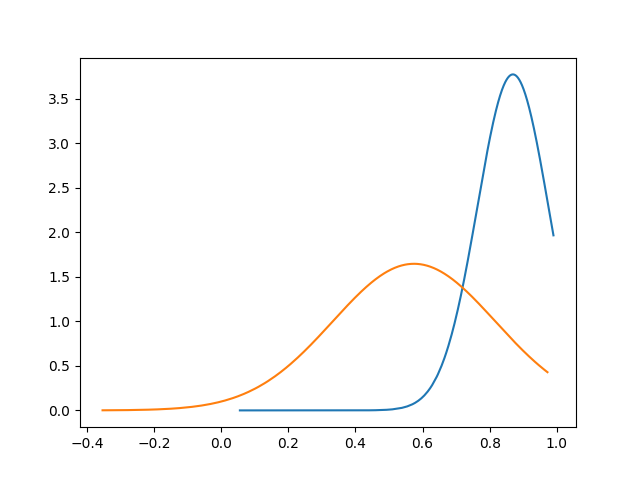
\includegraphics[width=0.45\textwidth]{clone_distribution}
	\caption{Plot of probability mass function (PMF) of cosine similarity - The blue bars indicate the PMF of cosine similarity of the cloned pairs. The yellow bars are for the non-cloned pairs.}
	\label{fig:clone_distribution}
\end{figure}

We extract all the expressions, the statements and the methods of each project in our training set, then we manually defined ground truth elements pair. We normalized each extracted code fragment, so called the token stream. We calculate the vector representation of the token stream in 2 different ways.

\textbf{Vector averaging} (avg): by averaging token vectors for all tokens in the token stream.

\textbf{Vector averaging with tf-idf} (avg-tfidf): a weighted average of the token vectors, where the weights are defined by the TF-IDF scheme. More precisely, the vector representation of a token stream \textit{s} is:

\begin{displaymath}
v_{s} = \frac{1}{|s|} \sum_{t \in s} IDF_{t}v_{t}
\end{displaymath}

where \begin{math}IDF_{t} \end{math} is the inverse document frequency of t, and \begin{math}|s|\end{math} denotes the number of tokens in the token stream. Here, the TF part of the TF-IDF scheme is taken into account by the sum over t \begin{math}\in\end{math} s. \begin{math}IDF_{t} \end{math} of a token can be calculates as:
\begin{displaymath}
IDF_{w} := log \frac{1 + N}{1 + N_{w}}
\end{displaymath}
where N is the total number of token streams and \begin{math}N_{w}\end{math} is the number of token streams containing token w, and 1 is added to avoid division by 0. In the experiments, we use all the data set \textbf{\textit{per language}} to compute the \begin{math}IDF_{t} \end{math}.

We take the vector representation of token stream from the source language as the query to rank the most similar token stream in the same group of the target language based on Euclidean distance. We also use the MAP score to evaluate this task.


\begin{figure*}[t!]
	\centering
	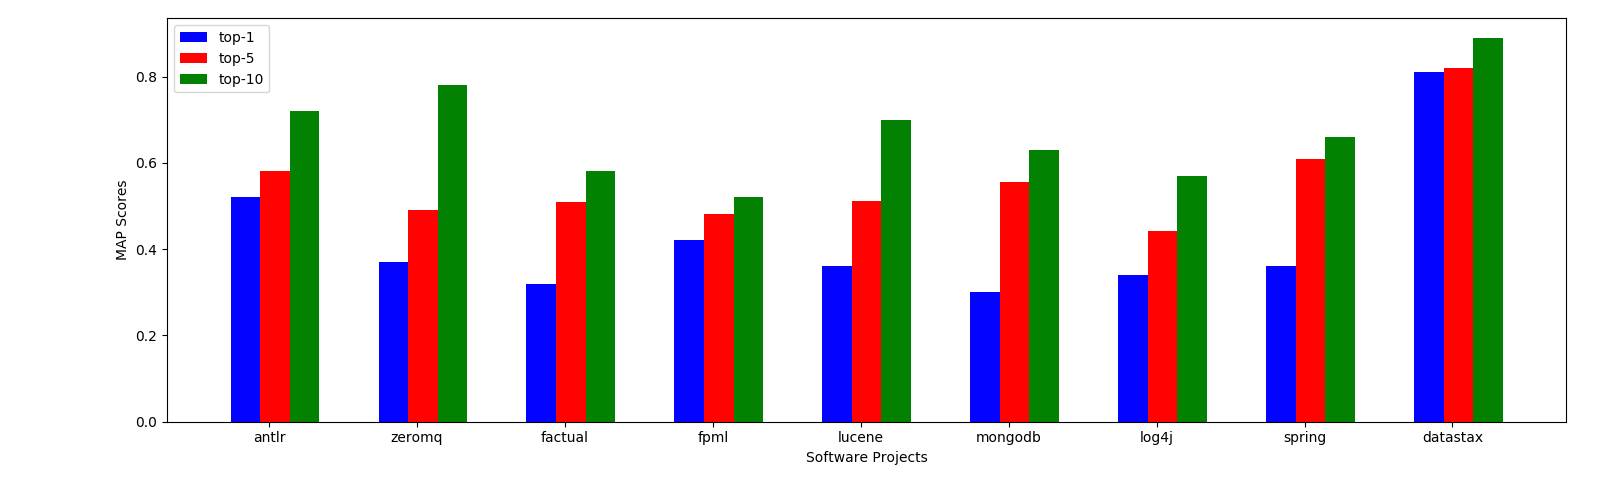
\includegraphics[width=1.05\textwidth]{top_k}
	\caption{Top-k queries for method-level mapping task, k = 1,5,10. The vector representation in this figure is calculated by avg-tfidf.}
	\label{fig:top_k}
\end{figure*}

\subsubsection{Clone detection}
To evaluate the impact of our model on real world tasks, we apply our approach into the diff dataset from (Cheng at al., 2016)\cite{cheng2017clcminer} for clone detection. The dataset contains 2000 pairs of diff, one diff is from C\# and the other is from Java, each pair has been labeled either cloned or non-cloned. 

For each diff, we perform normalization step (Section 3.1) to get the normalized version of the diff, also called as "token stream". We also get the vector representation of the token stream in 2 ways: vector averaging and vector averaging with tfidf.

Once we get the vector representations for each pair of diff o, we calculate the similarity between vectors by using the cosine similarity metric. We plot the probability mass function (PMF) of cosine similarity for all pairs of diff in Figure \ref{fig:clone_distribution}. Here we want to find the decision boundary to separate the 2 groups: cloned and none-cloned. 





\subsection{Result and Analysis}
\subsubsection{Tokens mapping}
To have a better visualization for the vector representation of tokens, here we use t-Distributed Neighbor Embedding (t-SNE) \cite{maaten2008visualizing}, a technique for dimensionality reduction that is particulary well suited for the visualization of high-dimensional datasets. Figure \ref{fig:tsne} shows a visualization of shared embedding for some similar tokens between C\# and Java, each pair of similar tokens are close together, e.g \textit{\textbf{if (\text{C\#})}} should be closest to \textit{\textbf{if (Java)}} and clusters with similar functionality should be located close to each other than other clusters, e.g the \textit{\textbf{if}} cluster should be closer to the \textit{\textbf{for}} cluster because both \textit{\textbf{if}} and \textit{\textbf{for}} are control statement.



Table \ref{tab:dataset} shows some example of top 5 most similar tokens once we take a token in the source language and find the most similar tokens in the target language, we demonstrate with some tokens that are supposed to be similar in bilingual languages.
\begin{table}
	
	\label{tab:nearest_neighbor_token_sample}
	\resizebox{\columnwidth}{!}{
		\begin{tabular}{cccc}
			
			
			\multicolumn{1}{c}{readonly(C\#)}  & \multicolumn{1}{c}{exception(Java)} & \multicolumn{1}{c}{lock(C\#)} &
			\multicolumn{1}{c}{package(Java)} \\
			\hline
			Java & C\# & Java & C\# \\
			\hline
			final & throw & lock & namespace  \\
			private & exception & synchronized & using \\
			static & throwable  & open & system \\
			extends & catch & checkpoint & sealed\\
			decl & finally & held & class\\
			
			
	\end{tabular}}
	\caption{Nearest neighbor tokens - shown are the top 5 nearest tokens when we take the vector of a word from the source vector space as the query to find the nearest neighbors in the target space, as measured by the Euclidean distance.}
	
\end{table}


Table \ref{tab:tokens_matching_top_k} shows the result when querying for 1-nearest neighbors, 3-nearest neighbors, 5-nearest neighbors, respectively.

\begin{table}
	
	
	
	\begin{tabular}{c|cc|cc|cc}
		
		\hline
		\multicolumn{1}{c}{}  &
		\multicolumn{2}{c}{1-NN}  &
		\multicolumn{2}{c}{3-NN}  & \multicolumn{2}{c}{5-NN} \\
		\hline
		& C\# & Java & C\# & Java & C\# & Java \\
		\hline
		MAP & 0.859 & 0.852 & 0.886 & 0.857 & 0.901 & 0.864 \\    
		
	\end{tabular}
	
	\medskip  
	\caption{Mean Average Precision for different top-k queries, k = 1,3,5. } 
	\label{tab:tokens_matching_top_k}
\end{table}


\subsubsection{Elements mapping}

Table \ref{tab:elements_mapping} shown the MAP score for top-5 query of the elements mapping task per project. The TF-IDF weighting scheme improves the result significantly in all projects and for any direction, from C\# to Java and from Java to C\#. The performance improvement of tfidf scheme is present more obvious in Figure \ref{fig:avg_vs_tfidf}. In Figure \ref{fig:top_k}, we show the MAP score result for the methods mapping task for top-k queries (k = 1,5,10), the vector representations in Figure \ref{fig:top_k} are calculated by \textit{avg-tfidf}.








\subsubsection{Clone Detection}
Figure \ref{fig:clone_distribution} shows the probability mass function (PMF) of cosine similarity (COSIM) for all pairs of diff. The blue curve indicates the PMF of the cloned pairs, The yellow curve is for the non-cloned pairs. The x-axis is the COSIM value. The y-axis shows the probability distribution of an x-value. The COSIM of the non-cloned pairs ranges from -0.4 to 0.8 and most of them assemble equally from 0.3 to 0.7, while the COSIM of cloned pairs ranges from 0.6 to 1 and most of them assemble equally from 0.8 to 1.

Because of this difference in COSIM distribution between cloned and non-cloned pairs, there exists a decision boundary to separate them, then this task becomes a classification problem. The COSIM is the only feature for this classification model. We use these well-known classifiers: Logistic Regression, Support Vector Machine and Random Forest to evaluate this problem. For per-project's pairs, we use 10-fold validation to evaluate the performance of the classification model.

To prove that the normalization step provides a better representation of tokens, we do the same task for the "non-normalization" version of the data set. In Table \ref{tab:clone_detection}, there are 2 parts, the first part is the classification result when we apply the normalizing step into the training data, the second part is for the "non-normalization" version.





\begin{table*}
	
	
	\resizebox{\textwidth}{!}{
		\begin{tabular}{c|cc|cc|cc|cc|cc|cc}
			
			
			Classifier & \multicolumn{4}{c|}{LR}  & \multicolumn{4}{c|}{RF} & \multicolumn{4}{c}{SVC Poly} \\
			\hline
			
			Baseline& \multicolumn{2}{c|}{Norm} & \multicolumn{2}{c|}{Non-Norm} & \multicolumn{2}{c|}{Norm} & \multicolumn{2}{c|}{Non-Norm}& \multicolumn{2}{c|}{Norm} & \multicolumn{2}{c}{Non-Norm}\\
			
			\hline
			Metric& Precision & Recall & Precision & Recall& Precision & Recall& Precision & Recall& Precision & Recall& Precision & Recall\\
			
			\hline
			antlr & 82.22 &83.44 &72.10 & 75.01 &80.12 &84.15 & 77.83 &73.22 &80.73 &81.40 &80.23 &75.15 \\
			cordova & 80.84 &83.44 &71.15 &74.18 &81.33 &81.98 & 78.15 &73.14 &83.51 &83.87 &77.49 &81.39 \\
			factual & 85.33 &86.92 &80.11 &70.09 &83.80 &82.42 & 71.40 &66.77 &80.02 &83.45 &74.12 & 80.55 \\
			lucene & 82.98 &84.56 &78.29 &81.76 &83.45 &87.43 & 74.28 &78.29 &81.06 & 80.92 &70.65 &79.82 \\
			zeromq & 79.59 &80.25 &77.50 &67.78 & 81.01 &83.49 &68.79 &69.90  &81.45 &86.18 &66.80 &78.49 \\
			spring & 84.23 &83.21 &80.12 &75.23 &82.76 &83.20 & 74.29 &72.86 &75.32 &85.19 &73.45 &76.29 \\
	\end{tabular}}
	
	\bigskip
	\caption{Clone detection result - shown are the precision and recall for the clone detection task. We extract the pairs of diff for each project. The cosine similarity between the diffs of each pair is served as the feature for the classification model. The Logistic Regression(LR), Random Forest (RF), and Support vector machine with the polynomial kernel (SVM Poly) are chosen as the classifiers for this problem. 10-fold validation is used to evaluate the models, we calculate precision and recall for each fold and calculate the average precision and average recall for all folds. The normalization versions produces significantly better result than the non-normalization.}
	\label{tab:clone_detection}
	
\end{table*}

\section{Discussion}
\subsection{Thread of validity}

The key part of our approach is the normalizing step to add more semantic features into the training data. This step is mostly based on srcML \cite{collard2011lightweight} to get the XML tag of the code elements. The tags represent the elements' kind. At this moment, srcML support 4 languages, they are: \texttt{C, C++, C\#} and \texttt{Java}. Then the generalizability of our approach serves these languages.

\subsection{Design choice}
\label{sub:designchoicde}


In this section, we want to discuss the choice of our normalization step discuss why the semantic keywords can produce better token representations. 

Let us consider a case of the key-value pair data structure. In C\#, the most commonly used library for this purpose is the \textit{Dictionary}, there are also some variances in C\#, eg. \textit{OrderedDictionary, KeyValuePair, Entry, etc}. On the other hand, usually the \textit{Map} are used but there are also a lot of variances in naming such data structure in Java, eg. \textit{HashMap}, \textit{LinkedHashMap}, \textit{KeyValuePair}, \textit{Entry}, \textit{SimpleKeyValue} etc. The developer uses difference variances of these libraries due to different requirements of performance, but the main purpose is to store data in the key-value style. This lead to the problem that once we collecting the aligned files and perform unsupervised token alignment task, there is a high likelihood that the \textit{dictionary} does not align with \textit{map}, and leads to the bad consequence that their vector representation can be very dissimilar. Consider these examples:
\begin{lstlisting}
new Dictionary ==> call new dictionary
new HashMap    ==> call new hash map
new Entry      ==> call new entry
new KeyValuePair      ==> call new key value pair
\end{lstlisting}

In the above examples, the normalization step (Section \ref{sub:normalization}) transform the code to create a new instance of key-value data structure source code (either in C\# or Java) to a normalized version. we add the keyword \textit{call} because the constructor of the object will be called.

Recall the intuition of Word2Vec, Word2Vec using large amounts of unannotated plain text to learn relationships between words automatically, a word is represented as a vector and the vector of words appeared in the same context are usually close to each other in the vector space. In our case, the \textit{call(C\#)} and \textit{call(Java)} are used to predict the context of these tokens {dictionary(C\#), entry(C\#), map(Java), entry(Java),pair(C\#), pair(Java)} (we ignore the others token in this example), then all of these tokens should be located somewhere around the two \textit{call}. The \textit{call} in this case act as a catalyst to reduce the difference in the similarity of these tokens. Moreover, it also acts as a \textit{\textbf{centroid}} to assemble tokens that \textit{supposed to be appear in the same context} into some region. In this case, the tokens are \{dictionary, map, pair, entry\}, as considering for both languages. Taking Figure \ref{fig:mapping_explain} as an example, both the \textit{call(C\#)} and \textit{call(Java)} are acted as the centroid of the others. With this, we somehow reduce the difference in semantic meanings between these tokens by clustering them into some region instead of letting them float sporadically in the vector space.
\begin{figure}[t!]
	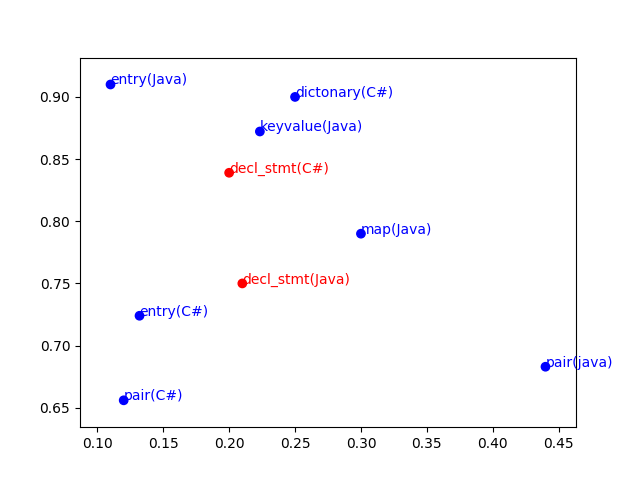
\includegraphics[width=0.45\textwidth]{mapping_explain}
	
	\caption{The \textit{call(C\#)} and \textit{call(Java)} acts as centroid to assemble tokens that appear in the same context into a region}
	\label{fig:mapping_explain}
	\medskip
\end{figure}

\subsection{Tokens mapping}
Here we want to discuss some cases that not produce good AP score in the token mapping task. Consider the case "\texttt{:}" in C\#. The top 8 Java tokens once taking "\texttt{:}" as the query are \texttt{\{this, constructor, case, throw, extends, weight, implements, require\}}. 

In C\#, the "\texttt{:}" usually appears in multiple contexts, it is used:

\begin{description}
	\item [$\bullet$] To separate a class name from its base class or interface implementations in class definitions or in generic constraint definitions. For example: 
	
	\texttt{public class Foo : Bar \{ \}}
	\item [$\bullet$] Indicating how to call another constructor on the current class or a base class's constructor prior to the current constructor. For example: 
	
	\texttt{public Foo() : base() \{ \}}
	\item [$\bullet$] To specify attribute targets. For example: \texttt{public Foo() : base() \{ \}}
	\item [$\bullet$] As part of a ternary expression.For example:
	
	\texttt{var a = b ? c : d;}
	\item [$\bullet$] As part of a switch case statement. For example:
	
	\texttt{switch(foo) \{ case bar: break; \}}
	\item [$\bullet$] As part of a goto label. For example:
	\texttt{goto Bar;}
	
\end{description}

With such multiple contexts, it is very difficult to distinguish between them because there are so many potential contexts that the token "\texttt{:}" may appear, this leads to a consequence that the token alignment step does not produce correct alignment for these tokens. There are quite some noises in the 10-nearest neighbor's result, they are some developer-defined token with semantic keyword added in our training phase (eg, constructor) and the language keywords (\texttt{extends} and \texttt{implements}), which supposed to belong to top 2 in results. An approach to this problem is to define the mapping between similar tokens as the initial alignments for the BiSkip model. With that, this becomes a semi-supervised problem, where we already have partial alignments initially. We leave this as a part of our futures works.

\subsection{Semantic Composition}
The TF-IDF weighting scheme improves the result of elements mapping and clone detection task significantly. Because this scheme penalizes the token that is so common, multiply this score to the vector representation of a token can reduce the "strength" of some common tokens which overwhelmed the others, hence affect the representation of the whole composition. For example, consider the case in Figure, the token \textit{identifier}, which is the semantic feature we added in the normalization step. This token appears too much in the statement, thus the vector of \textit{identifier} overwhelm the others, which contains more important information. The TF-IDF scheme shows the usefulness in penalizing such cases.

The statements and the methods are usually the compositions of some meaningful sub-elements, some may be more important, while the other may be less. By averaging all of the tokens, we treat all tokens the same while ignoring the importance of each token in statements, or methods. TF-IDF weighting scheme does a better job to treat the strength of tokens in a better way, but for some case, the result is not satisfied enough. The TF-IDF scheme is based on the bag-of-words model, therefore it does not capture the position of the token in the text, semantics, co-occurrences in different. Here we want to consider the importance of a token in within statements or methods. Our goal is to represent a program as a hierarchical layer of granularity, as in Figure \ref{figure:softwarelayers}, then the vector of a parent element will be represented as some aggregation of the vector its children. In Natural Language, Socher \cite{socher2011parsing} represents a sentence as a parse tree and use the recursive neural networks (RNN) to capture both the syntactic and compositional-semantic information of parent node by merging its children node. Yang \cite{yang2016hierarchical} considers a document as a hierarchical structure (words form sentences, sentences form a document) and represents this structure as a hierarchical neural network.



We have seen that at character-level, the neural network model is capable of writing Linux kernel after learning the entire Linux-based source code, as described in \cite{Karpathy}. Thus the neural-based technique to generate source code is an achievable target. We believe that our work can be a good foundation for a neural network-based programming language translation, which is a more sophisticated task. 

\section{Conclusion and Future Work}
This work proposes an approach to learn the mappings between programming languages. By utilizing the alignment of files across languages, we can learn the alignment of tokens in an unsupervised manner, then we can learn the share embeddings between languages. The shared embeddings are able to bring the benefits to learn the semantic cross-lingually. We show that we can map most of the elements between languages accurately under a fine-grained manner. This can be served as a foundation for more complicated tasks, such as programming language translation. In the future, we want to extend our approach in highly dissimilar languages, e.g Haskell, Scala, Ruby, etc. We also aim to build a hierarchical architecture that can aggregate a better representation of complicated compound elements.



\begin{acks}
	
\end{acks}
